\newpage
\section{Manuel Utilisateur}
\label{sec:manuel}

\subsection{D�roulement d'une partie}
\label{sec:deroulement}

\paragraph{}Une partie commence � minuit le 1er janvier 2017.

\subsubsection{Mode Normal}
\label{sec:deroulementnormal}
\paragraph{}Au d�but d'une partie en mode normal, il est possible de choisir son niveau de difficult� entre:
\begin{itemize}
\item Niveau Easy: Un seul personage sur la map
\item Niveau Normal: Trois personnes sur la map
\item Niveau Hard: Cinq personnes sur la map
\item Niveau Pro: Quinze personnes sur la map (le maximum)
\end{itemize}

\begin{figure}[H]
	\centering
		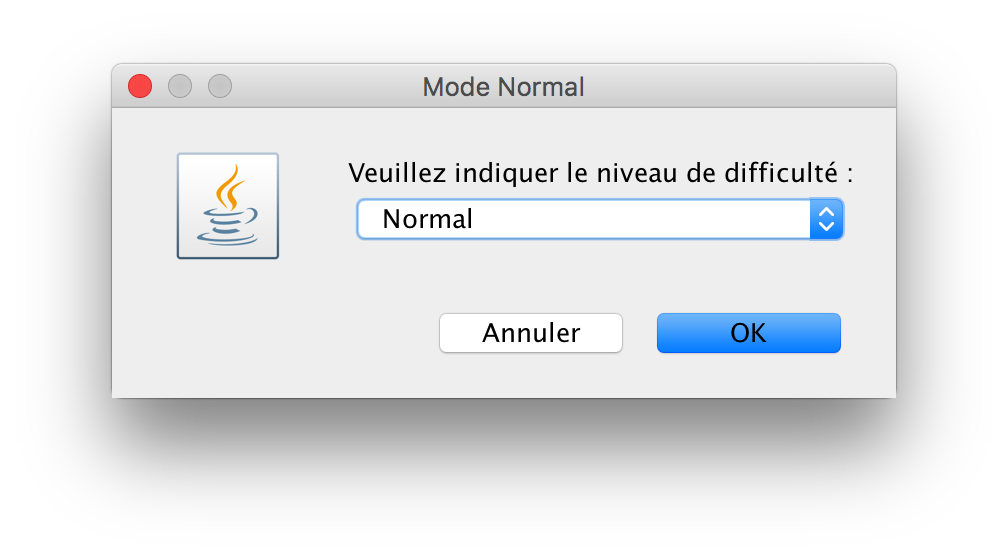
\includegraphics[width=0.5\textwidth]{images/niveau_normal.png}
		\caption{Fen�tre de selection de niveau en mode normal}
	\label{fig:nivnormal}
\end{figure}

\begin{figure}[H]
	\centering
		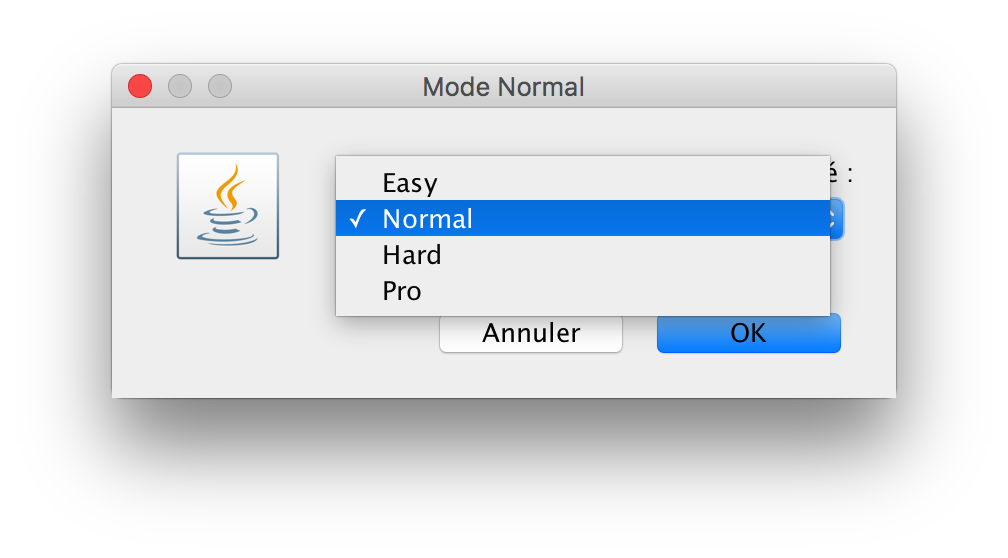
\includegraphics[width=0.5\textwidth]{images/niveausel_normal.png}
		\caption{Les differents niveau en mode normal}
	\label{fig:nivselnormal}
\end{figure}

\paragraph{}L'objectif du joueur est de faire survivre sa population le plus longtemps possible en influent sur le comportement des personnages. Un personnages meurt lorsqu'une de ces jauge (Emotion, Money, Family) arrive � 0. La partie s'arr�te quand il n'y a plus de personnages en vie.

\subsubsection{Mode Autonome}
\label{sec:deroulement_auto}
\paragraph{}En mode autonome le joueur ne peut influer sur le comportement des personnages. Le mode autonome est simulation de l'evolution d'une population dans un environnement urbain. L'utilisateur peut choisir le nombre de personnages pr�sent dans la population lors de la simulation, au d�but de la partie. Le nombre de personnages en mode autonome peut aller de 1 � 60.
\begin{figure}[H]
	\centering
		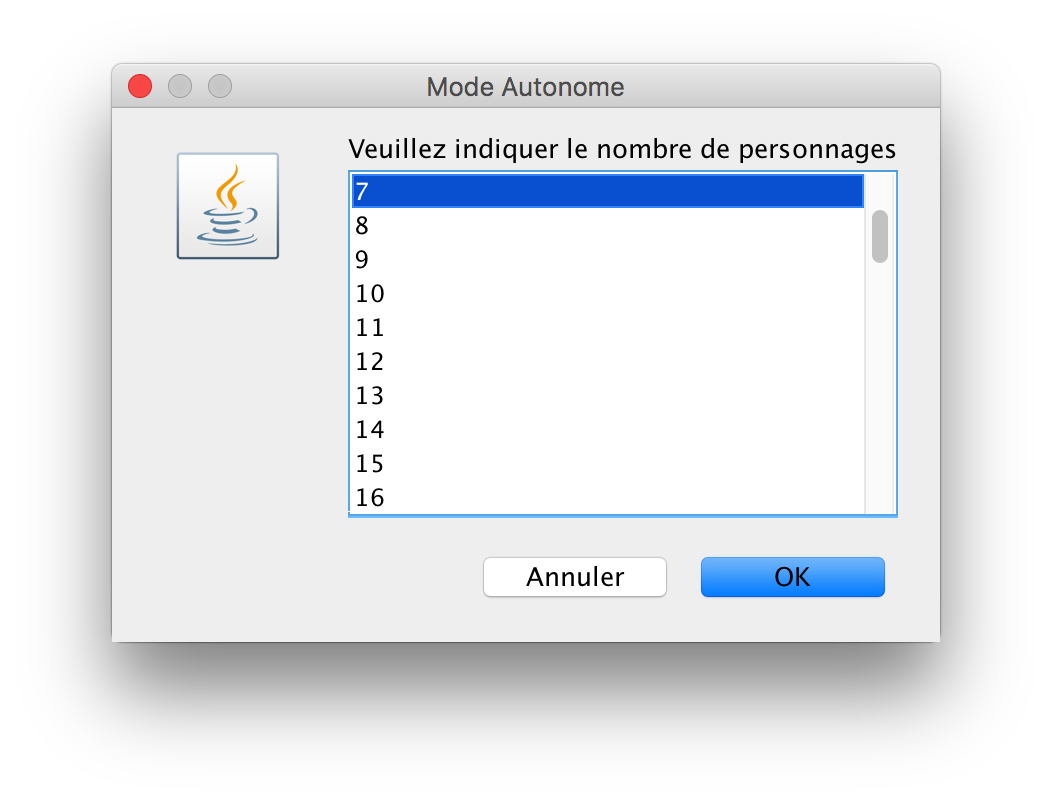
\includegraphics[width=0.5\textwidth]{images/niveau_auto.png}
		\caption{La s�lection du nombres de personnages en mode autonome}
	\label{fig:nivselauto}
\end{figure}

\paragraph{}La partie, en mode autonome, ne se fini jamais. En effet lorsqu'une des jauges d'un personnages arrive � 0, ce personnage d�m�nage et commence une nouvelle vie, jusqu'� arriver � vivre une vie stable.


\subsection{Manuel de l'IHM}
\label{sec:manIHM}

\begin{figure}[H]
	\centering
		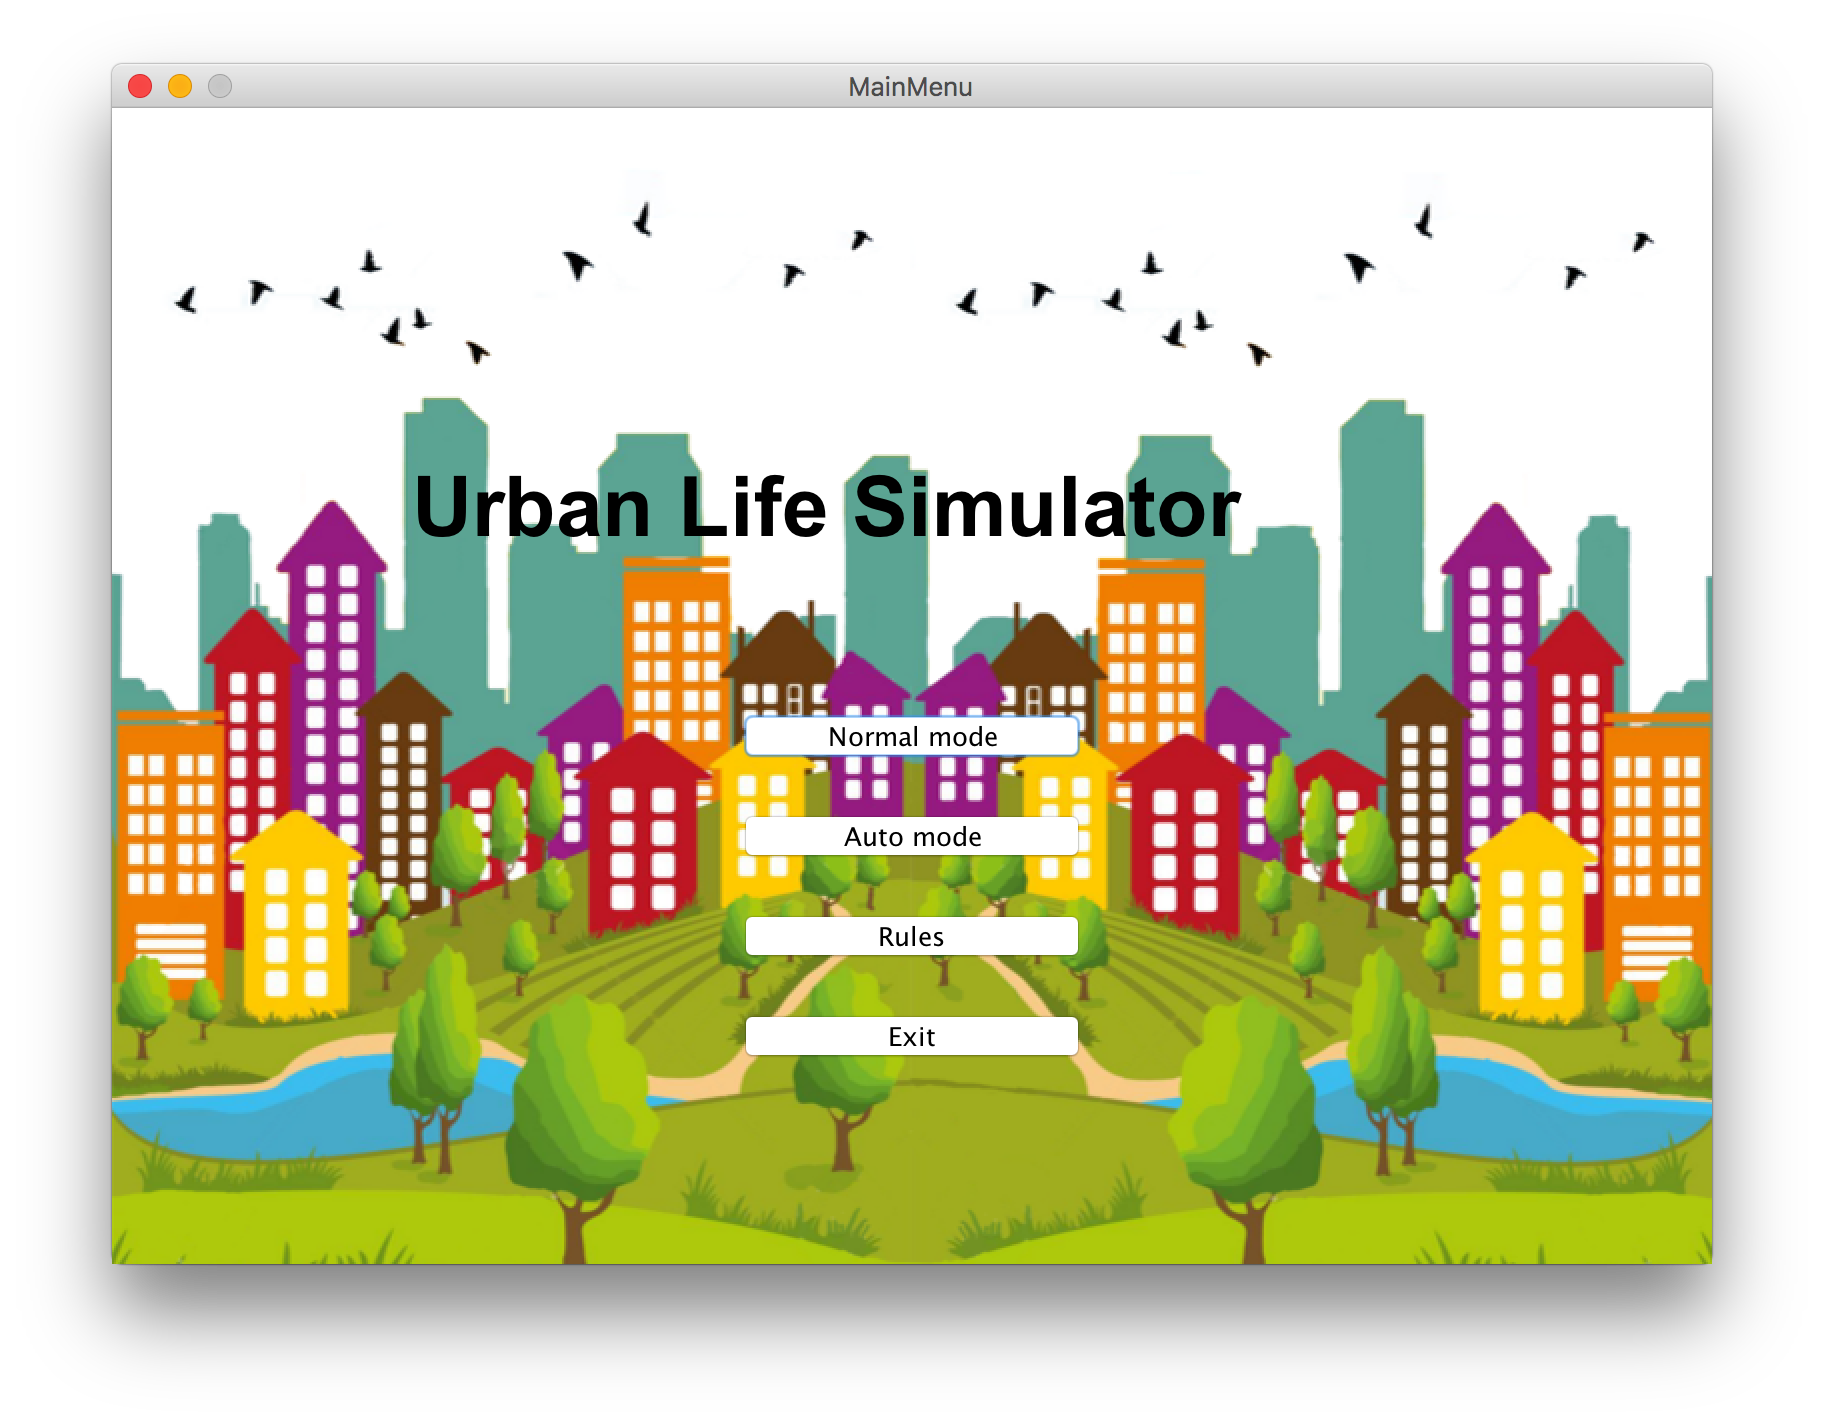
\includegraphics[width=0.75\textwidth]{images/mainmenu.png}
		\caption{Menu principal}
	\label{fig:mainmenu}
\end{figure}

\begin{figure}[H]
	\centering
		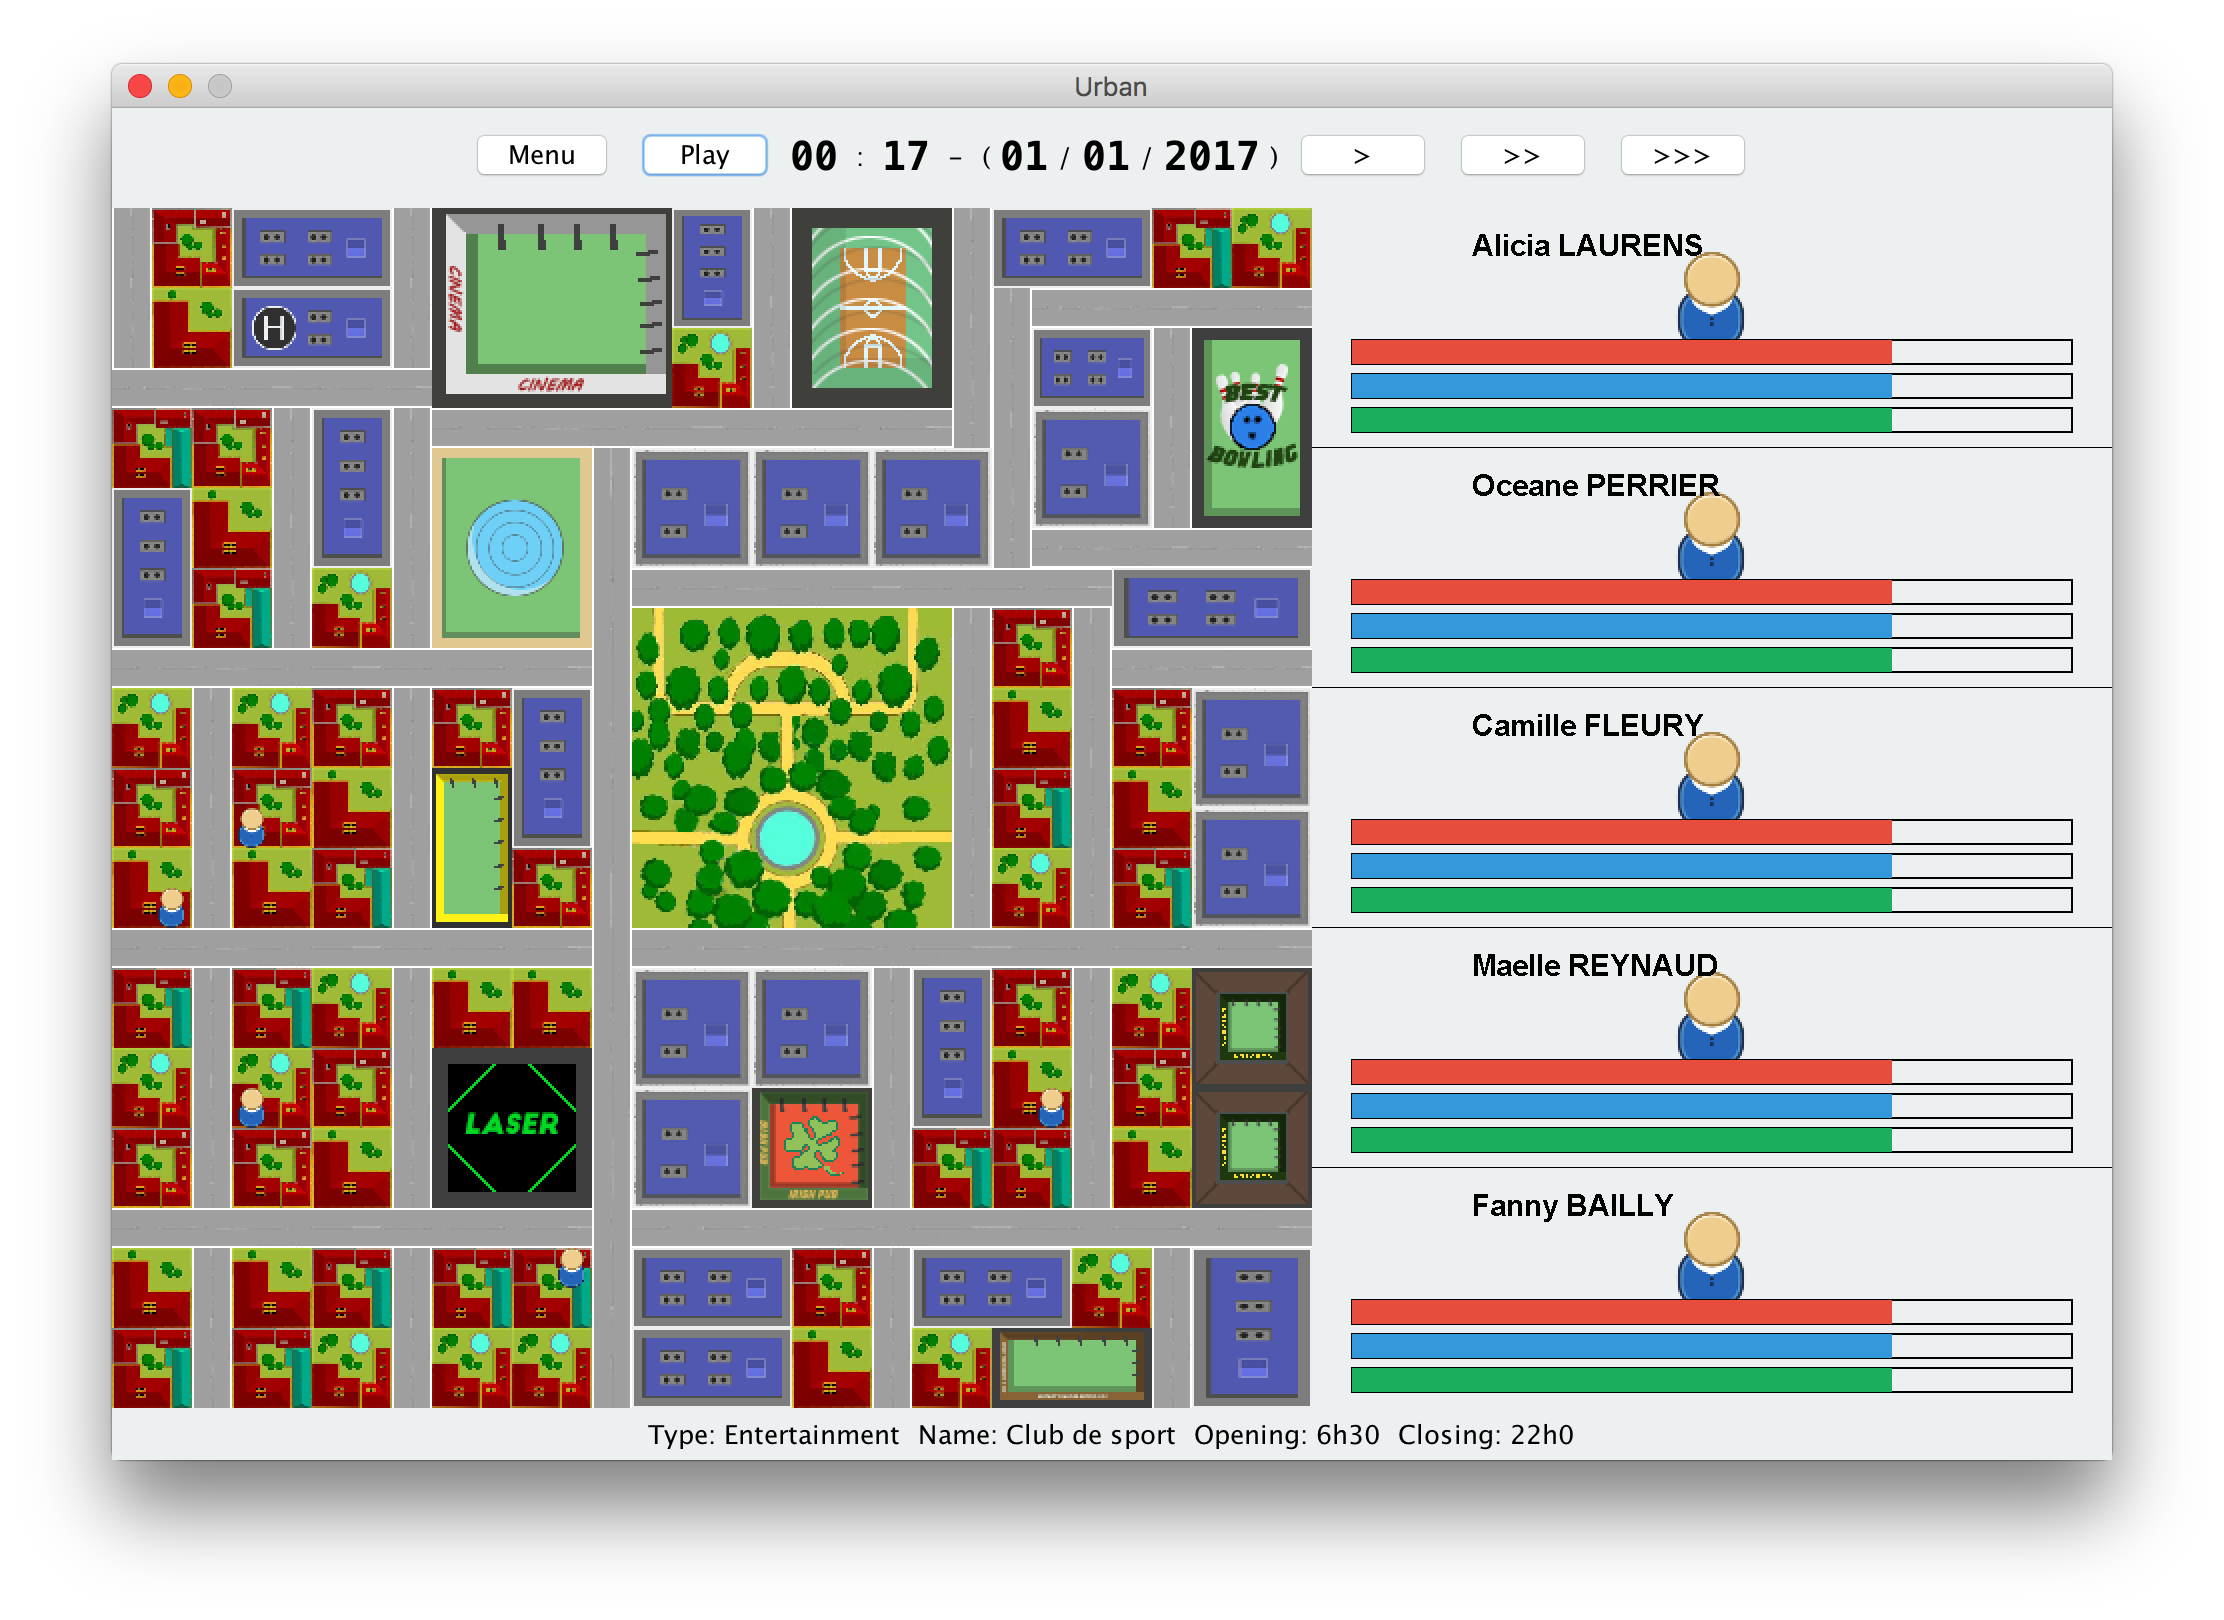
\includegraphics[width=0.75\textwidth]{images/ingame_1.png}
		\caption{IHM du jeu}
	\label{fig:ingame1}
\end{figure}


\subsubsection{Information des Infrastructures}
\label{sec:maninfrainfo}
\paragraph{}Pour afficher les informations d'une infrastructure, l'utilisateur peut double-cliquer sur n'importe qu'elle infrastructure sur la map.
\begin{figure}[H]
	\centering
		
\includegraphics[width=0.75\textwidth]{images/maninfrainfo.png}
		\caption{Information des infrastructures}
	\label{fig:maninfreinfo}
\end{figure}

\subsubsection{Information de l'Horloge}
\label{sec:manclock}
\paragraph{}Cette partie, en plus de contenir les informations sur l'horloge rafraichie automatiquement, contient 5 boutons:
\begin{itemize}
\item Bouton menu: permet de revenir au menu principal (Met fin � la partie)
\item Bouton Play/Pause: Permet de stopper l'horloge et de la faire reprendre
\item Bouton Speed: 3 niveau disponible permettant de r�gler la rapidit� de l'horloge
\end{itemize}
\begin{figure}[H]
	\centering
		
\includegraphics[width=0.75\textwidth]{images/manclock.png}
		\caption{Information sur l'horloge}
	\label{fig:manclock}
\end{figure}

\subsubsection{La Map}
\label{sec:manmap}
\paragraph{}La Map est un affichage de la situation de la population dans son environnement, � l'instant T, elle ne poss�de pas de bouton permettant de la controler.
\begin{figure}[H]
	\centering
		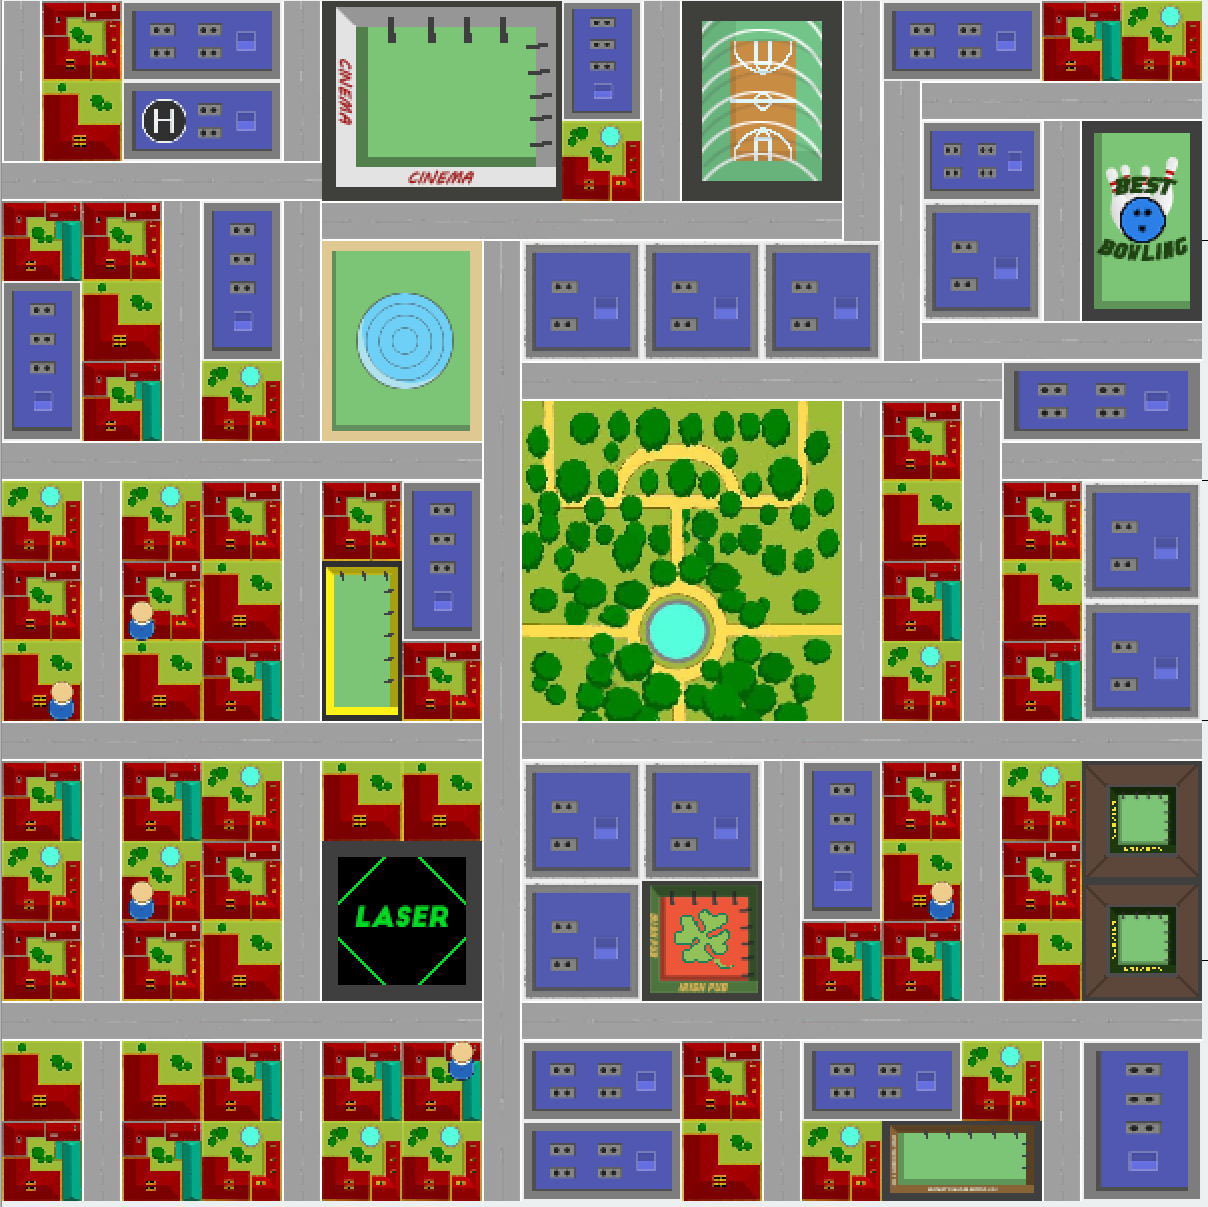
\includegraphics[width=0.75\textwidth]{images/manmap.png}
		\caption{Affichage de la Map}
	\label{fig:manmap}
\end{figure}

\subsubsection{Liste des personnages}
\label{sec:manlist}
\paragraph{}
